\chapter{Data} \label{Chap3}

\section{Dataset}

\subsection{Site Description and Overview}

The North Wyke Farm Platform comprises three hydrologically isolated grazed-grassland catchments,
each drained independently and instrumented with an Eddy Covariance flux tower: Tower 2, Tower 4,
and Tower 9. Each catchment is farmed as a distinct beef-cattle system and is treated throughout
this dissertation as an independent modelling unit -- soil moisture, meteorological, and flux
variables are never pooled across catchments without an explicit tower identifier, since doing so
would mix physically distinct fields (Section 3.1.2). EC towers report half-hourly flux estimates;
supporting meteorological and soil sensors report at 15-minute resolution; livestock location
counts are recorded daily per catchment. Catchment area varies across the three sites and underlies
the livestock-density (livestock-units per hectare) features used throughout Chapters~\ref{Chap4}
and~\ref{Chap6}. The EC record used in this dissertation spans 2018 to 2023 for training and
evaluation, with 2024 reserved as a held-out window (Section 3.2.1).

\subsection{Captured Metrics / Data Sources}

Three categories of source data are used as gap-filling features in this dissertation. EC flux and
micrometeorological variables (30-minute resolution) provide the target (FCH4) alongside its
established covariates: incoming shortwave radiation, air temperature, vapour pressure deficit,
friction velocity (USTAR), wind speed, and soil heat flux. One naming detail is worth flagging as a
concrete data-handling due-diligence point: shortwave radiation was initially expected under a
\texttt{SW\_IN\_} column-naming pattern by analogy with standard FLUXNET conventions, but is
recorded at NWFP under \texttt{SWIN\_1\_1\_1} instead -- a reminder that every column mapping in
this dataset was verified directly against the data rather than assumed from convention. Soil
moisture and soil temperature (15-minute resolution) are recorded per catchment and are never
averaged across towers (Section 3.1.1). Livestock location counts (daily, per catchment, per
species) provide the livestock-density features identified as the dominant CH\textsubscript{4}
driver in Chapters~\ref{Chap4}--\ref{Chap6}. Two further data sources exist in the raw NWFP export
but were explored during EDA and not adopted as gap-filling features: 17-parameter catchment
water-quality chemistry and raw animal body-condition scores, both retained in the raw data but
outside this dissertation's feature scope. Bodyweight, fertiliser-application recency, and
catchment flow are used later in this dissertation (Chapters~\ref{Chap5} and~\ref{Chap6}) and are
introduced at that point rather than catalogued here, since they play no role in gap-filling itself.

\section{Exploratory Data Analysis}

Two properties of the raw data motivate the modelling pipeline that follows: FCH4 is severely
incomplete (Section 3.2.1), and the dataset spans multiple measurement frequencies that must be
reconciled onto a common temporal index before any model can be trained (Section 3.2.2).

\subsection{Availability of Data per Year}

FCH4 target completeness varies sharply across the three towers, computed directly from the
consolidated hourly record: Tower 4 is missing 56.5\% of hourly observations, Tower 9 is missing
75.0\%, and Tower 2 is missing 88.5\%. Tower 2's incompleteness is dominated by a single, confirmed
structural cause rather than instrument noise: a 1,675-day continuous gap from May 2019 to January
2024, corresponding to a genuine land-use change on the Red farmlet (field NW002) from permanent
pasture to arable cultivation, during which the EC tower's flux footprint no longer represented
grazed grassland. This gap is treated as a real missing-data mechanism, not something to be
gap-filled through, and is returned to as a modelling limitation in Chapter~\ref{Chap7}. Separately,
2024 exists in the raw data but is deliberately withheld from all training and validation as the
project's final held-out evaluation window, consistent with the temporal train/test/held-out split
adopted throughout this dissertation.

\begin{figure}[htbp]
\centering
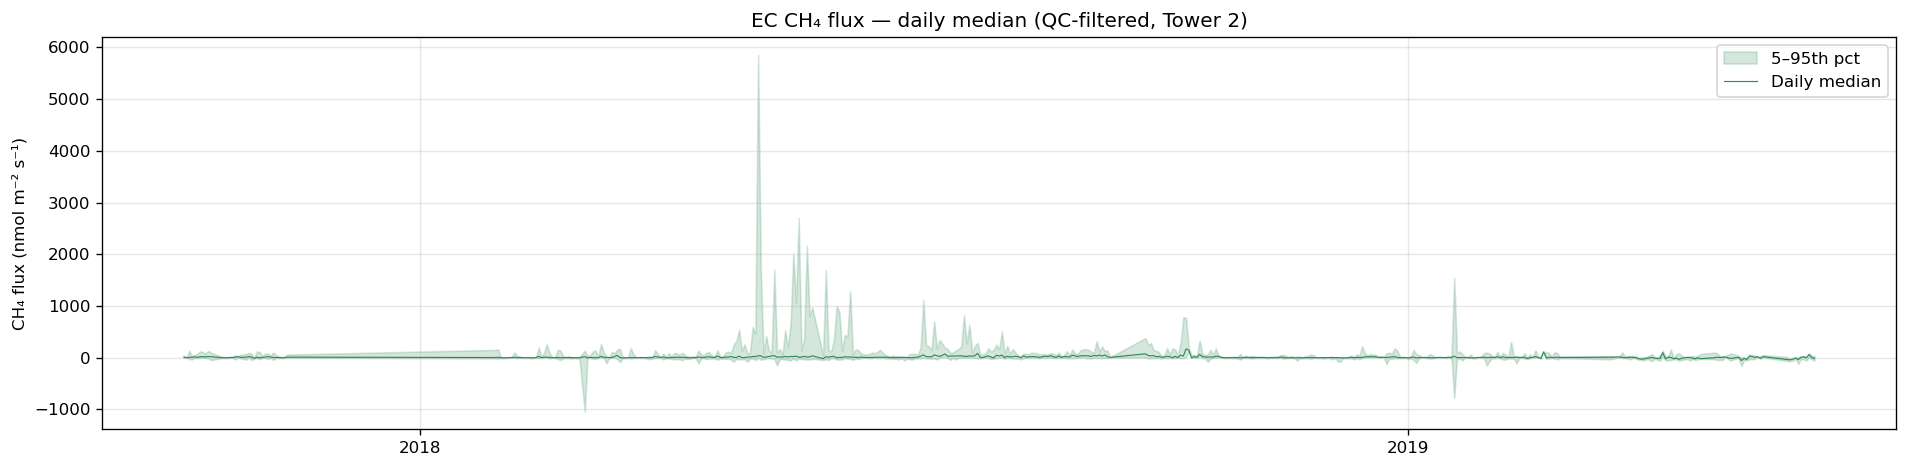
\includegraphics[width=0.85\textwidth]{Figures/ch3_t2_timeseries.png}
\caption{Tower 2 EC CH4 flux, daily median with 5th--95th percentile band -- illustrating the
spike-dominated character of the target and the years-long stretch of near-total absence following
the 2019 land-use conversion.}
\end{figure}

\begin{figure}[htbp]
\centering

\includegraphics[width=0.85\textwidth]{Figures/ch3_t2_availability_heatmap.png}
\caption{Tower 2 FCH4 data availability (\% valid half-hours) by year and month, showing the
1,675-day gap from mid-2019 through the end of 2023.}
\end{figure}

\begin{figure}[htbp]
\centering
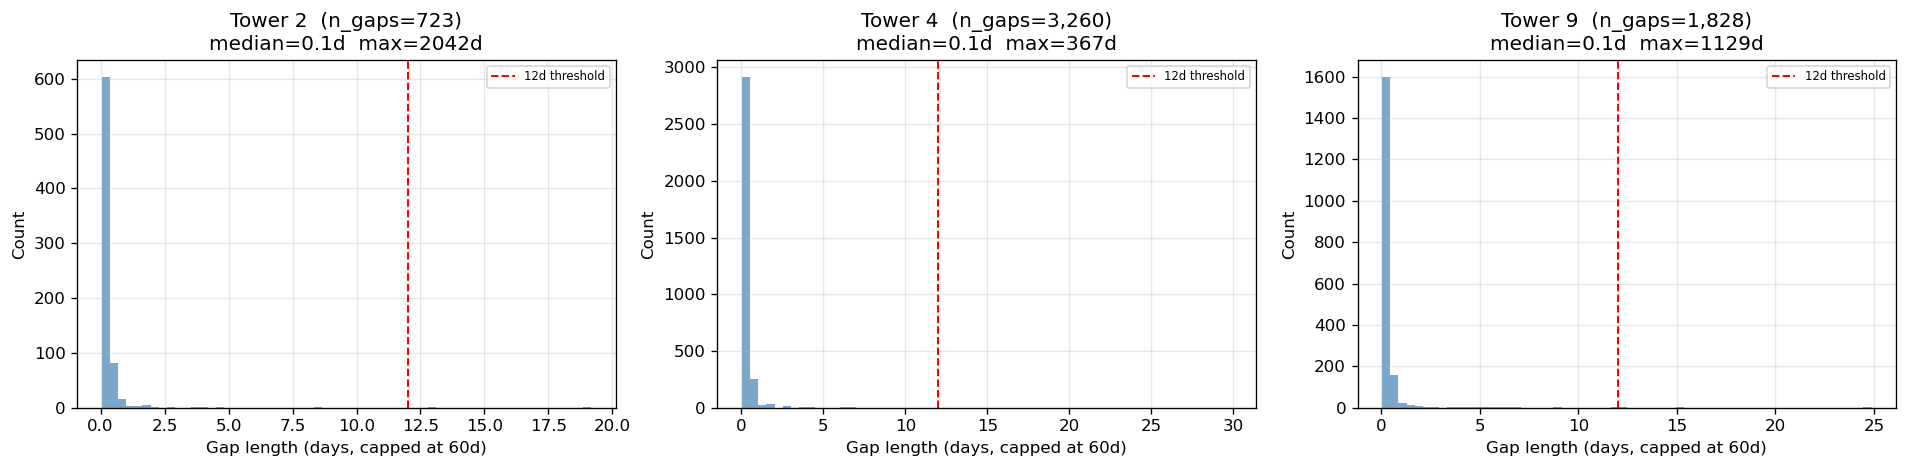
\includegraphics[width=\textwidth]{Figures/ch3_gap_length_distribution.png}
\caption{Distribution of FCH4 gap lengths by tower. The 12-day (288-hour) dashed threshold marks
the longest artificial-gap scenario used throughout the gap-filling evaluation protocol
(Chapter~\ref{Chap4}).}
\end{figure}

\FloatBarrier

% \subsection{Different Levels of Granularity Within the Dataset}

% The dataset combines three native sampling frequencies: 30-minute EC flux and micrometeorological
% variables, 15-minute soil and flow measurements, and daily livestock location counts. All sources
% are consolidated onto a common 1-hour index prior to any modelling step, aggregating sub-hourly
% variables and forward-filling daily livestock counts within each day. This single consolidated
% hourly table is the common starting point for gap-filling (Chapter~\ref{Chap4}), forecasting
% (Chapter~\ref{Chap5}), and scenario projection (Chapter~\ref{Chap6}).

\subsection{Temporal Analysis and Dimensionality Reduction}

Beyond standard correlation and autocorrelation/partial-autocorrelation (ACF/PACF) diagnostics used
throughout to characterise FCH4's temporal dependence structure, two nonlinear
dimensionality-reduction methods were applied to the environmental feature space: UMAP and Time-lagged
Independent Component Analysis (TICA). TICA originates in molecular dynamics, where it identifies
the slowest-evolving collective coordinates of a trajectory; unlike UMAP, which preserves static
neighbourhood structure, TICA maximises autocorrelation over an explicit time lag, making it the
more natural lens for a temporally-structured environmental record and the method preferred here.
TICA was fitted per-tower on contiguous temporal segments at a 24-hour lag; UMAP and t-SNE
embeddings were computed on a reproducible, tower-balanced sample (1,000 rows per tower), each
coloured by tower identity, season, and FCH4 observed/missing status. A local 15-neighbour
label-agreement test against chance found that towers separate well above chance (+0.13 to +0.18)
and seasons separate even more strongly (+0.18 to +0.23), but FCH4-observed and FCH4-missing hours
are barely distinguishable from chance (+0.04 to +0.05) -- missing-target hours occupy essentially
the same environmental neighbourhoods as observed ones. This is a reassuring result specifically
for gap-filling: it supports interpolation from available training conditions rather than raising a
covariate-shift concern, since missingness in FCH4 does not correspond to a distinct region of
environmental-feature space.

Building on this diagnostic, a fold-safe consensus feature-selection procedure was implemented
using TICA loadings together with UMAP and t-SNE permutation importance, computed independently
per outer cross-validation fold (30 folds: 3 towers $\times$ 5 scenarios $\times$ 2 repetitions) to
avoid leakage, and combined into a single consensus ranking. This produced a remarkably stable
result: a 6-variable core -- soil temperature, soil moisture, air temperature, vapour pressure
deficit, wind speed, and soil heat flux -- was selected in every single fold, precipitation was
excluded in every fold, and friction velocity (USTAR) was selected inconsistently (30\% of folds).
This consensus ranking underpins the feature sets used in the gap-filling benchmark of
Chapter~\ref{Chap4}.

\begin{figure}[htbp]
\centering
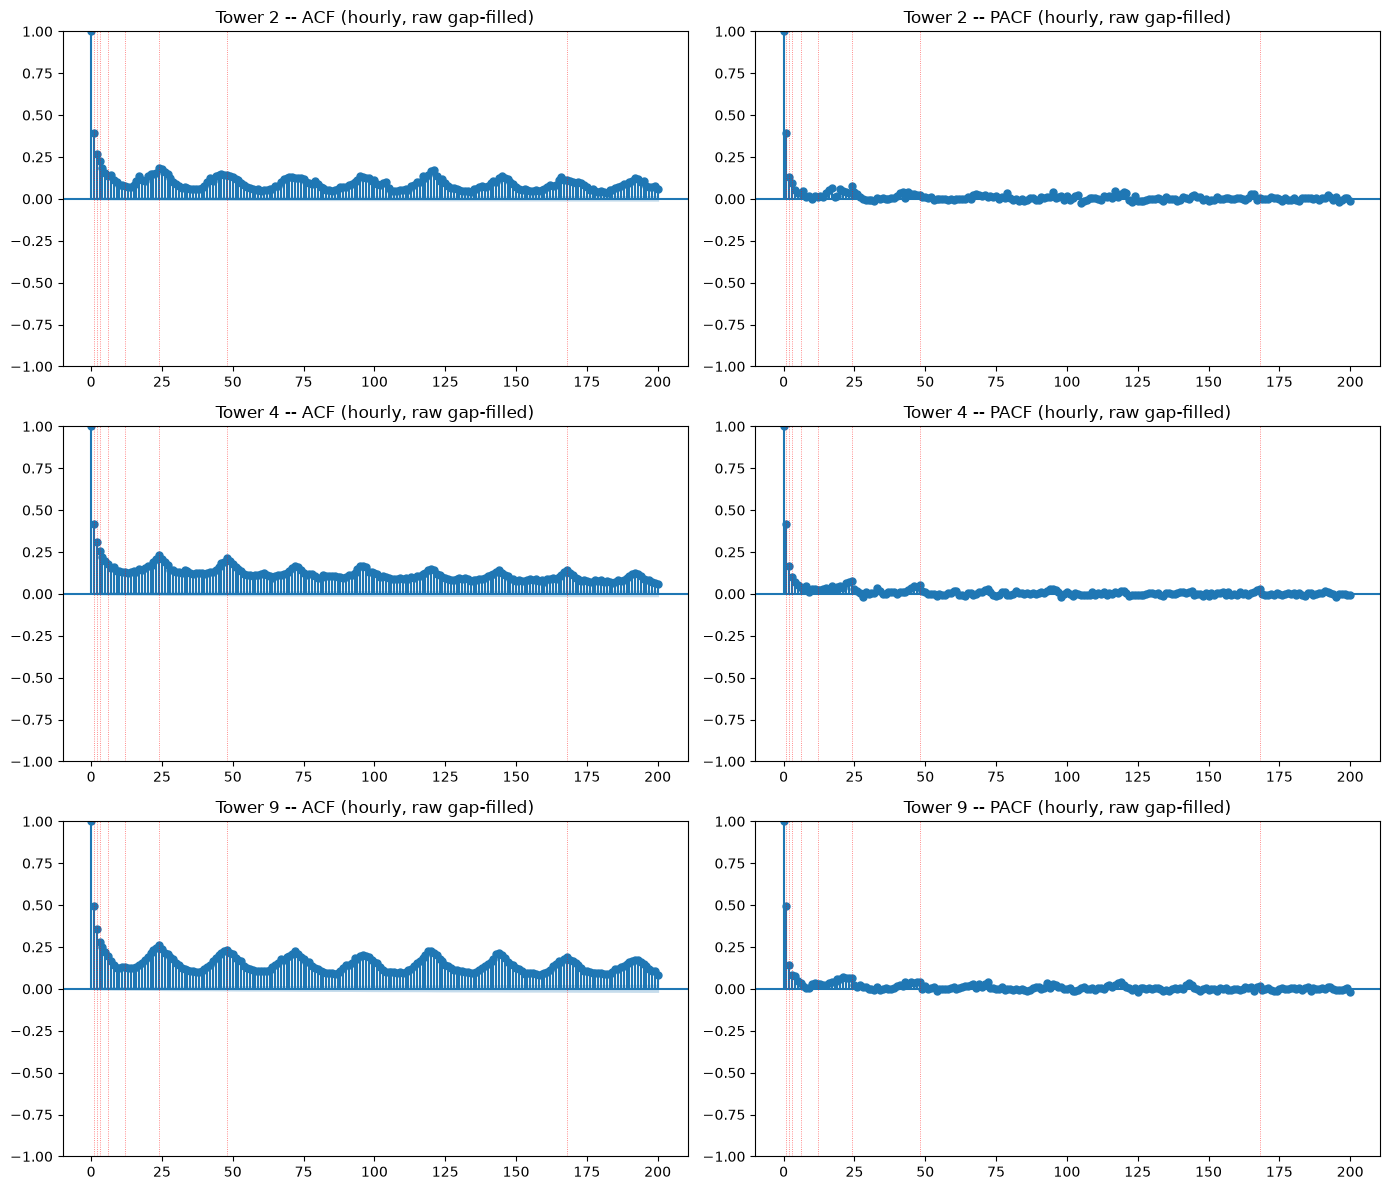
\includegraphics[width=\textwidth]{Figures/ch3_acf_pacf_hourly.png}
\caption{Hourly ACF and PACF of FCH4 (raw gap-filled series) per tower, out to a 200-hour lag. The
diurnal periodicity is visible as repeating peaks in the ACF; PACF decays sharply after the first
few lags.}
\end{figure}

\begin{figure}[htbp]
\centering
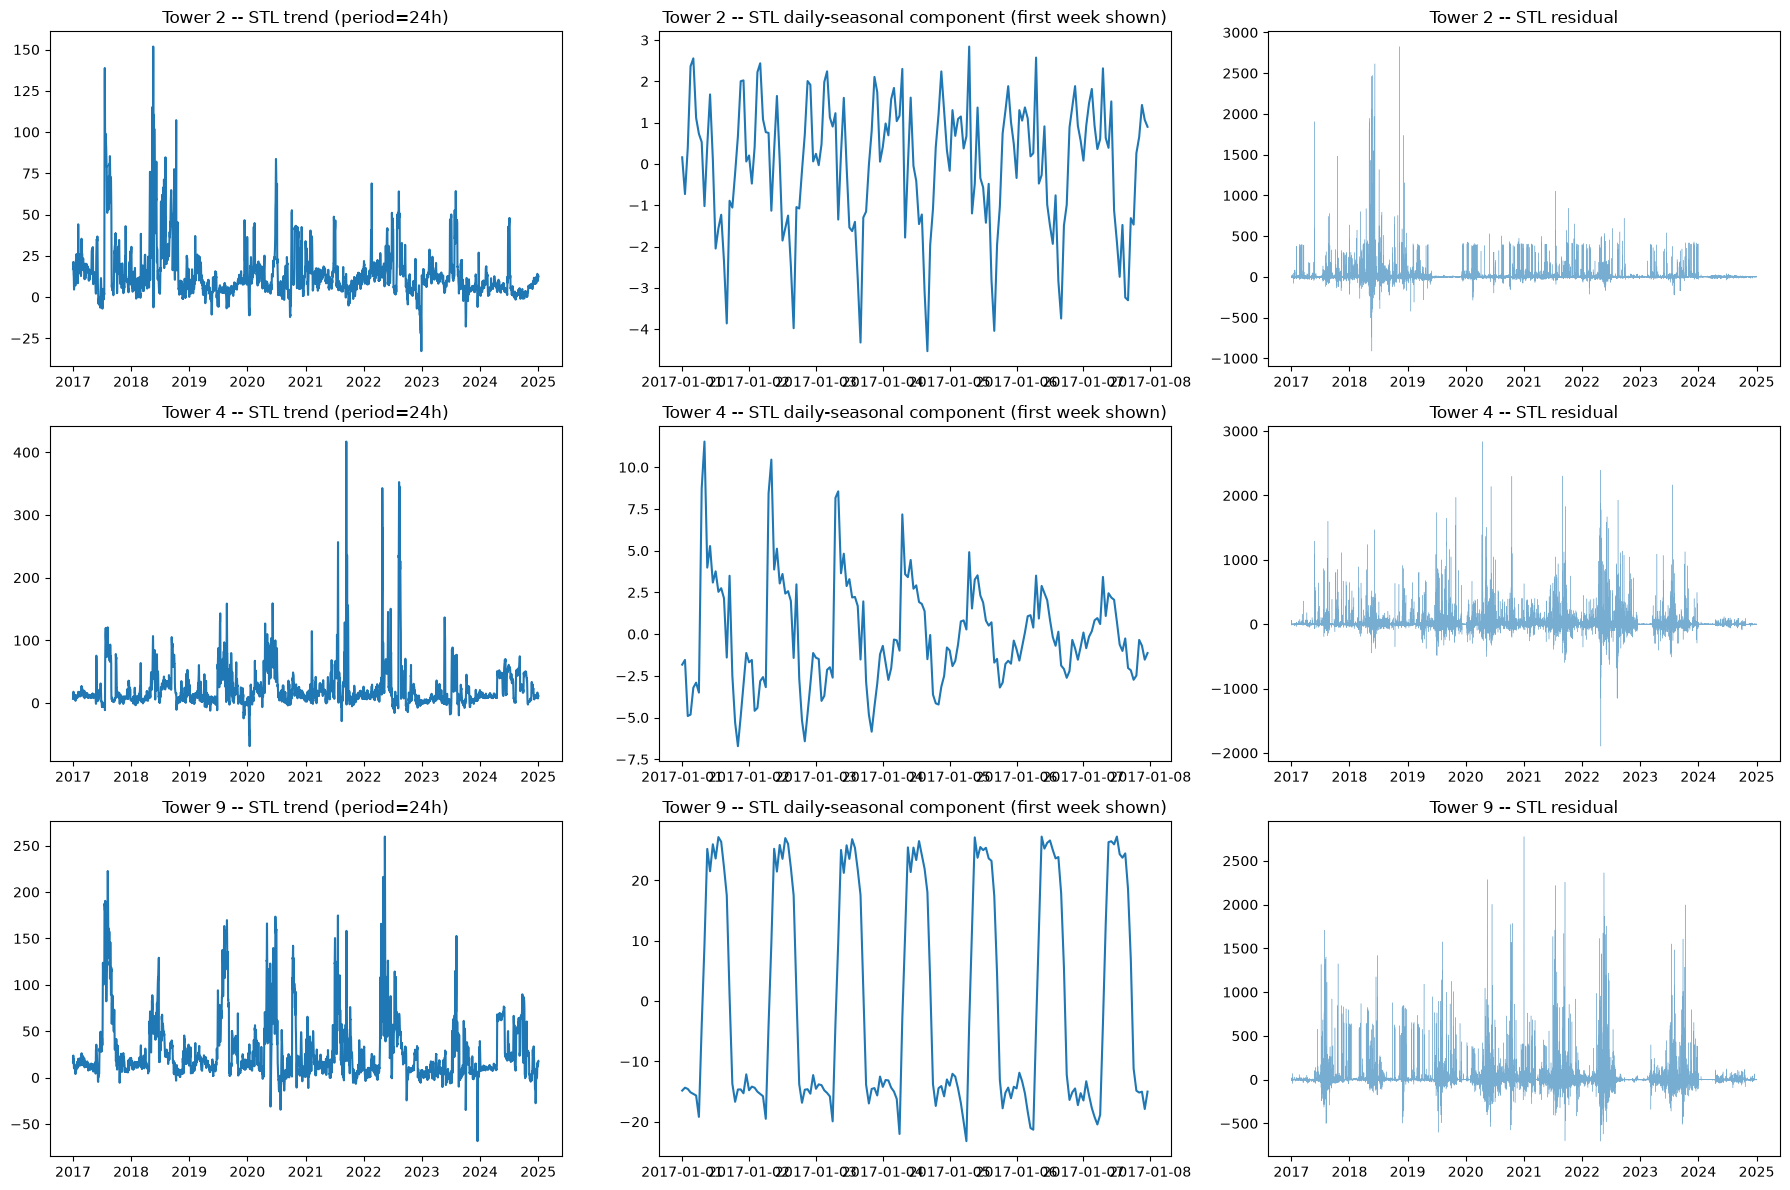
\includegraphics[width=\textwidth]{Figures/ch3_stl_decomposition.png}
\caption{STL decomposition of hourly FCH4 per tower (24-hour period): trend, daily-seasonal
component (first week shown), and residual.}
\end{figure}

\begin{figure}[htbp]
\centering
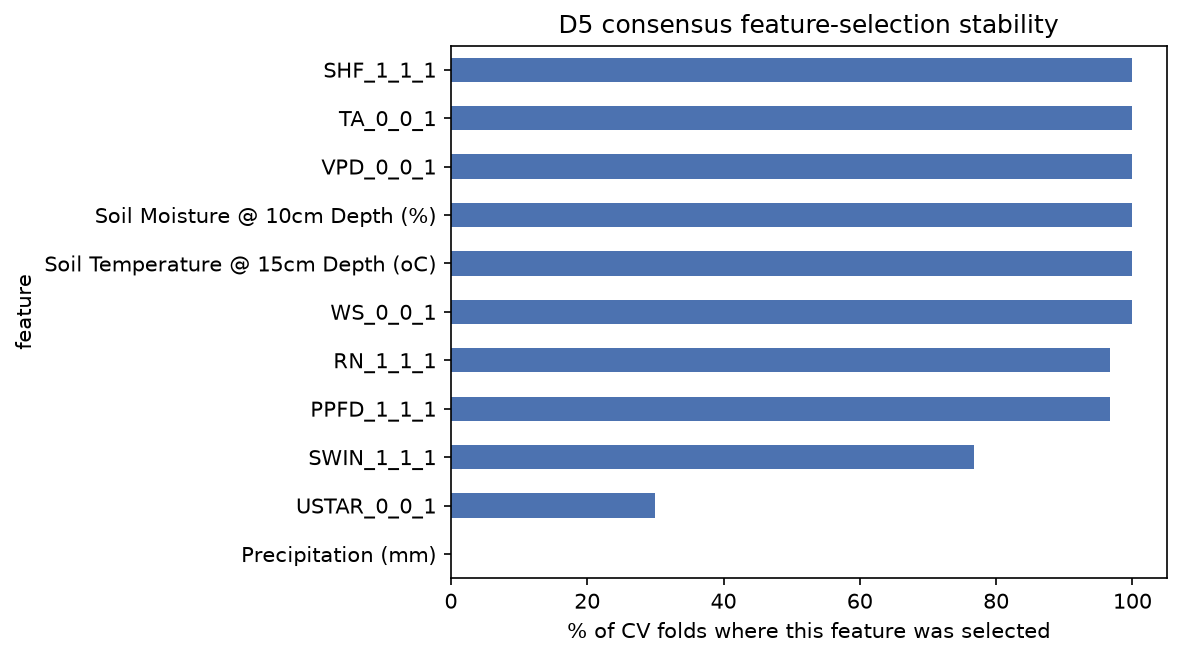
\includegraphics[width=0.75\textwidth]{Figures/ch3_tica_umap_selection_stability.png}
\caption{D5 consensus feature-selection stability: \% of cross-validation folds in which each
meteorological variable was selected by the combined TICA/UMAP/t-SNE consensus ranking.}
\end{figure}

\FloatBarrier

\section{Data Preprocessing Done}

\subsection{Gap-Filling}

Meteorological driver variables (as distinct from the FCH4 target itself, whose gap-filling is this
dissertation's primary contribution and is presented in full in Chapter~\ref{Chap4}) are gap-filled
using a Python reimplementation of REddyProc-style logic
(\texttt{src/data/reddyproc\_pipeline.py}, \texttt{mdc\_gapfill()}), combining Marginal
Distribution Sampling-style interpolation with a mean-diurnal-course fallback for extended gaps.
This is a direct reimplementation of the standard EC gap-filling logic in Python rather than an
invocation of the original R \texttt{REddyProc} package, which is not used anywhere in this
project's codebase.

\subsection{Data Correction, Truncation, and Filtering}

Two sensor-contamination issues were identified and corrected during preprocessing, both
significant enough to be treated as data-correction events rather than routine filtering. First, a
USTAR (friction velocity) contamination bug produced physically impossible readings as high as
1039.9 m/s, silently corrupting the mean-based gap-fill fallback during extended sensor blackouts.
A matching contamination pattern was identified in vapour pressure deficit (VPD). Both were traced
and corrected through a staged truncation fix applied to wind speed and air temperature inputs
upstream of the affected derived variables. These corrections were applied before the dimensionality-
reduction analysis of Section 3.2.3 and the gap-filling benchmark of Chapter~\ref{Chap4}, so results
reported in both chapters reflect the corrected data throughout.
